\documentclass[
  11pt,
  letterpaper,
  % addpoints,
  answers
]{exam}

\usepackage{../tarea}

\begin{document}
\begin{minipage}{0.42\textwidth}
    
\includegraphics[width=\textwidth]{../fcfm_die}
\end{minipage}
\begin{minipage}{0.53\textwidth}
\begin{center} 
\large\textbf{Clases Particulares} \\
\normalsize Prof.~Gonzalo Narváez.
\end{center}
\end{minipage}

\vspace{0.5cm}
\noindent
\begin{questions}

    \question{Resuelva el siguiente problema utilizando la carta de Smith. Se tiene una línea de transmisión de impedancia característica $Z_0 = \qty{75}{\ohm}$ y una carga $Z_l = \complexqty{70-40\ju}{\ohm}$. Se desea adaptar la carga a la línea de transmisión.}
    
    \begin{center}
      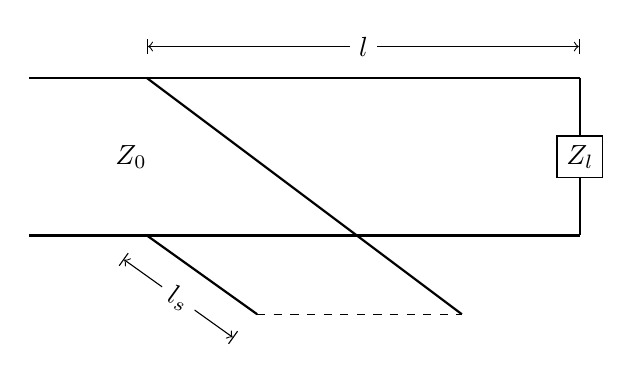
\begin{tikzpicture}
        % Línea de transmisión
        \draw[thick] (-4,1) -- (3,1); 
        \draw[thick] (-4,-1) -- (3,-1);
  
  
        %stub
        \draw[thick] (-2.5,1) -- (1.5,-2);
        \draw[thick] (-2.5,-1) -- (-1.1,-2);
  
        \draw[|<->|] (-2.5,1.4) -- (3,1.4) node[midway, fill=white] {$l$};
  
        \draw[|<->|] (-2.5-.3,-1-.3) -- (-1.1-.3,-2-.3) node[midway, rotate=-22, fill=white] {$l_s$};
        \draw[dashed] (-1.1,-2) -- (1.5,-2);
          
        %impedanciia Z_l
        \node[draw] (ZL) at (3,0) {$Z_l$};
        \draw[thick] (3,1) -- (ZL.north);
        \draw[thick] (3,-1) -- (ZL.south);

        
        \node at (-2.7,0) {$Z_0$};
      
    
      \end{tikzpicture}
      \captionof{figure}{Linea de transmisión en circuito abierto.}
      \label{fig:lt}
    \end{center}
    Para adaptar la Linea determine:
    \begin{parts}

        \part[3]{La distancia $l$ con tal de adaptar la parte real de la admitancia.}
    
        \part[4]{La distancia $l_s$ con tal de adaptar la parte imaginaria de la línea de transmisión tanto en corto circuito ($l_\text{s}^\text{cc}$) como en circuito abierto ($l_\text{s}^\text{ca}$).}
    
        \part[3]{Explique el proceso de adaptación.}
      \end{parts}
    
    \begin{solution}

        
      



    \end{solution}
    
  \end{questions}
\end{document}
